% THIS IS SIGPROC-SP.TEX - VERSION 3.1
% WORKS WITH V3.2SP OF ACM_PROC_ARTICLE-SP.CLS
% APRIL 2009
%
% It is an example file showing how to use the 'acm_proc_article-sp.cls' V3.2SP
% LaTeX2e document class file for Conference Proceedings submissions.
% ----------------------------------------------------------------------------------------------------------------
% This .tex file (and associated .cls V3.2SP) *DOES NOT* produce:
%       1) The Permission Statement
%       2) The Conference (location) Info information
%       3) The Copyright Line with ACM data
%       4) Page numbering
% ---------------------------------------------------------------------------------------------------------------
% It is an example which *does* use the .bib file (from which the .bbl file
% is produced).
% REMEMBER HOWEVER: After having produced the .bbl file,
% and prior to final submission,
% you need to 'insert'  your .bbl file into your source .tex file so as to provide
% ONE 'self-contained' source file.
%
% Questions regarding SIGS should be sent to
% Adrienne Griscti ---> griscti@acm.org
%
% Questions/suggestions regarding the guidelines, .tex and .cls files, etc. to
% Gerald Murray ---> murray@hq.acm.org
%
% For tracking purposes - this is V3.1SP - APRIL 2009

\documentclass{acm_proc_article-sp}

\usepackage{caption}
\usepackage{soul}
\usepackage{color}
\usepackage{url}
\usepackage{hyperref}
\usepackage{subfig}
\usepackage{graphicx}

\begin{document}
\title{Implementing Baum-Welch Algorithm}
\subtitle{Assignment 3}
%
% You need the command \numberofauthors to handle the 'placement
% and alignment' of the authors beneath the title.
%
% For aesthetic reasons, we recommend 'three authors at a time'
% i.e. three 'name/affiliation blocks' be placed beneath the title.
%
% NOTE: You are NOT restricted in how many 'rows' of
% "name/affiliations" may appear. We just ask that you restrict
% the number of 'columns' to three.
%
% Because of the available 'opening page real-estate'
% we ask you to refrain from putting more than six authors
% (two rows with three columns) beneath the article title.
% More than six makes the first-page appear very cluttered indeed.
%
% Use the \alignauthor commands to handle the names
% and affiliations for an 'aesthetic maximum' of six authors.
% Add names, affiliations, addresses for
% the seventh etc. author(s) as the argument for the
% \additionalauthors command.
% These 'additional authors' will be output/set for you
% without further effort on your part as the last section in
% the body of your article BEFORE References or any Appendices.

%\numberofauthors{3} %  in this sample file, there are a *total*
% of EIGHT authors. SIX appear on the 'first-page' (for formatting
% reasons) and the remaining two appear in the \additionalauthors section.
%
\numberofauthors{1}
\author{
	\alignauthor Caitlin Ross\\
	\affaddr{Computer Science Department, Rensselaer Polytechnic Institute} \\
	\email{rossc3@rpi.edu}
}
% There's nothing stopping you putting the seventh, eighth, etc.
% author on the opening page (as the 'third row') but we ask,
% for aesthetic reasons that you place these 'additional authors'
% in the \additional authors block, viz.

\date{30 July 1999}
% Just remember to make sure that the TOTAL number of authors
% is the number that will appear on the first page PLUS the
% number that will appear in the \additionalauthors section.

\maketitle

\begin{abstract}
Hidden Markov models (HMM) can be used to find CpG islands in an unannotated sequence.  Here we build a HMM using the Baum-Welch algorithm to estimate the transition and emission probabilities.  We have been given 10 DNA sequences that were generated using a two state HMM.  We implement the Baum-Welch algorithm and run the resulting program on these 10 sequences.  We find that the algorithm does appear to correctly estimate the transition and probability matrices.
\end{abstract}


\section{Problem Statement}
Hidden Markov models (HMM) can be used to find CpG islands in an unannotated sequence.  The Markov chain models that were explored in the last homework can be used to create a single model that can find CpG sequences of variable length.  Here we use a two state HMM.  For the HMM, we need to find the transition and emission probabilities.  The transition probabilities are the probabilities of either remaining in state or switching to the other state .  The emission probabilities are the probability of seeing a given symbol in that state.  The problem here is to implement the Baum-Welch algorithm in order to estimate the transition and emission probabilities of the given data set.  

\section{Methods}
This section describes the program developed to solve this problem and the math needed.

For our HMM we need to determine the transition probabilities $a_{kl}$, which is the probability of transition from state k to state l and is defined as
\begin{equation}a_{kl} = P(\pi_{i} = l |\pi_{i-1} = k)\end{equation}
We also need to find the emission probabilities of each symbol b when seen in state k, which is defined as
\begin{equation}e_{k}(b) = P(x_{i} = b | \pi_{i} = k)\end{equation}

The Baum-Welch depends on two other algorithms to assist in finding these probabilities.  The forward algorithm uses dynamic programming to find the probability that some state path could have produced the given sequence.  We find a matrix f, where each row represents a state.  We initialize $f_{0}(0) = 1$ and $f_{1}(0) = 0$.  Then for each state $l$, we have that
\begin{equation}f_{l}(i) = e_{l}(x_{i})\sum_{k}f_{k}(i-1)a_{kl}\end{equation}
for $i=1...L$ where L is the length of the sequence.  The termination condition is then
\begin{equation}P(x) = \sum_{k}f_{k}(L)a_{k0}\end{equation}
where $a_{k0}$ represents a transition from state k into the end state.  

The backward algorithm is similar but finds the posterior probabilities starting from the end of the sequence.  In this case, we find a matrix b, again where each row represents a state.  We initialize $b_{k}(L) = a_{k0}$ for each state k.  For each state k, we have that
\begin{equation}b_{k}(i) = \sum_{l}a_{kl}e_{l}(x_{i+1})b_{l}(i+1)\end{equation}
and that the termination condition is
\begin{equation}P(x) = \sum_{l}a_{0l}e_{l}(x_{1})b_{l}(1)\end{equation}
where $a_{0l}$ is the probability to start in state $l$.

For the Baum-Welch, we start off with random numbers generated for the emission probabilities, normalizing the values for each state.  For each sequence in the assign3.fasta file provided, we calculate $f_{k}(i)$ and $b_{k}(i)$ and add those contributions to the matrices A and E.  $A_{kl}$ represents the expected number of times that $a_{kl}$ is used and is formally defined as
\begin{equation}A_{kl} = \sum_{j} \frac{1}{P(x^{j})}\sum_{i}f_{k}^j(i)a_{kl}e_{l}(x^j_{i+1})b^j_{l}(i+1)\end{equation}
$E_{k}(b)$ is the expected number of times that letter b appears in state k and is defined as 
\begin{equation}E_{k}(b) = \sum_{j}\frac{1}{P(x^j)}\sum_{\{i|x^j_{i}=b\}}f_{k}^j(i)b_{k}^j(i) \end{equation}

Once that is done for each sequence in the data set, the new model parameters can be calculated by 
\begin{equation}a_{kl} = \frac{A_{kl}}{\sum_{l'}A_{kl'}}\end{equation}
and 
\begin{equation}e_{k}(b) = \frac{E_{k}(b)}{\sum_{b'}E_{k}(b')}\end{equation}

Finally the log likelihood of the model can be calculated by 
\begin{equation}\sum_{j\in{sequences}}\log{P(x_{j})}\end{equation}
where $P(x_{j})$ is the value returned from the termination step of the forward algorithm for sequence j.

The program uses the file \texttt{assign3.fasta}, which contains 10 DNA sequences that are each 300 bases long.  We know that the sequences were generated using a two state HMM, where one state is G-C rich and the other is A-T rich.  The program reads in this file and runs it through the Baum-Welch algorithm just described.  


\section{Results}
After running the program, we end with a log likelihodd of -4109.0229.  The estimated transition and emission matrices are shown in Tables 1 and 2, respectively.  As seen in the table, the HMM has correctly estimated that one state is A-T rich, and the other is G-C rich.  State 1 appears to be the A-T rich state and State 2 appears to be G-C rich.  

\begin{table}
\centering
\caption{Transition Matrix}
\label{posmat}
\begin{tabular}{|c|c|c|} \hline
 &State 1&State 2\\ \hline
State 1  &0.93885 &0.06115  \\ \hline
State 2  &0.10666  &0.89334 \\ 
\hline\end{tabular}
\vspace{1.8em}
\caption{Emission Matrix}
\label{negmat}
\begin{tabular}{|c|c|c|c|c|} \hline
 &A&C&G&T\\ \hline
State 1  &0.40383  &0.08516  &0.07901  &0.43199 \\ \hline
State 2  &0.12853  &0.39166  &0.35570  &0.12411 \\ 
\hline\end{tabular}
\end{table}

\section{Problems Encountered}
I did encounter some problems understanding the notation.  I followed the book closely, but some parts were confusing.  For instance, to calculate f, that starts with a 0 index, but the book assumes that the sequence is initially indexed at 1, so I encountered a lot of indexing issues.  I might still have some slight error in my code, but I appear to be close as the matrices do tend to go to expected values.  

%\begin{figure}[!b]
%	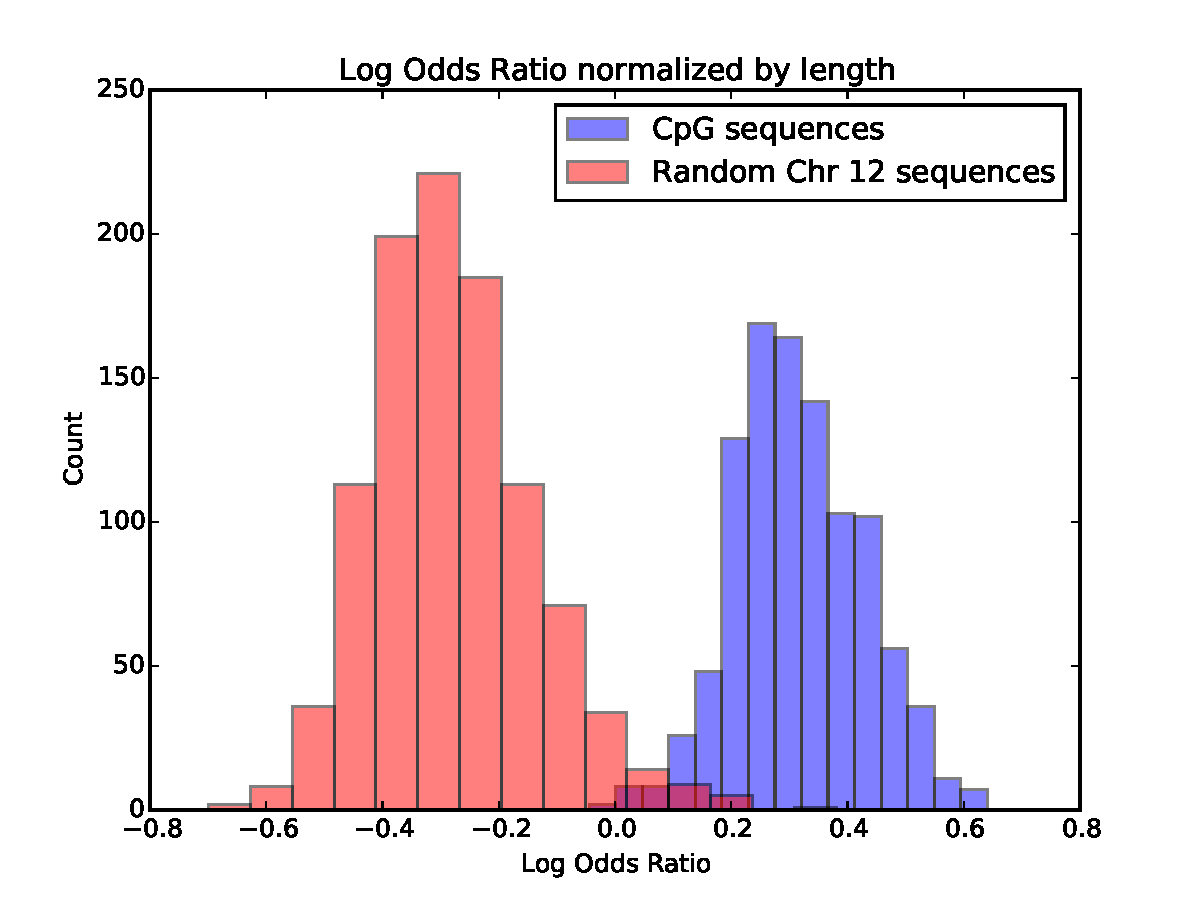
\includegraphics[trim={0 0 2cm 0}, clip,width=3.5in]{histogram.pdf}
%	\caption{Histogram of log odds ratios of the positive and negative test sets normalized for the length of the sequences}
%	\label{fig:hist}
%\end{figure}



%
% The following two commands are all you need in the
% initial runs of your .tex file to
% produce the bibliography for the citations in your paper.
\bibliographystyle{abbrv}
%\bibliography{sigproc}  % sigproc.bib is the name of the Bibliography in this case

% You must have a proper ".bib" file
%  and remember to run:
% latex bibtex latex latex
% to resolve all references
%
% ACM needs 'a single self-contained file'!
%
%APPENDICES are optional
%\balancecolumns

\balancecolumns
% That's all folks!
\end{document}
